\subsection{Funktionsstyringsmodulet}
\label{sub:styringsmodul}

Funktionsstyringsmodulet har til opgave at instantiere og kontrollere de moduler som udgør specifikke funktionaliteter for brugeren.

\subsubsection{Funktionalitet}
\label{ssub:hovedmodul_funktionalitet}

Når en bruger har været igennem en succesfuld validering fra loginmodulet, bliver brugeren sendt videre til funktionsstyringsmodulet. Dette modul fungerer som skelettet for de omkringliggende moduler. Brugeren bevæger sig derfor hele tiden rundt indenfor dette moduls rammer, indtil brugeren ønsker at logge ud af programmet. funktionsstyringsmodulet bør altid instantiere et default modul med basal information til brugeren.

\subsubsection{Implementation}
\label{ssub:hovedmodul_implementation}

\begin{figure}
  \centering
  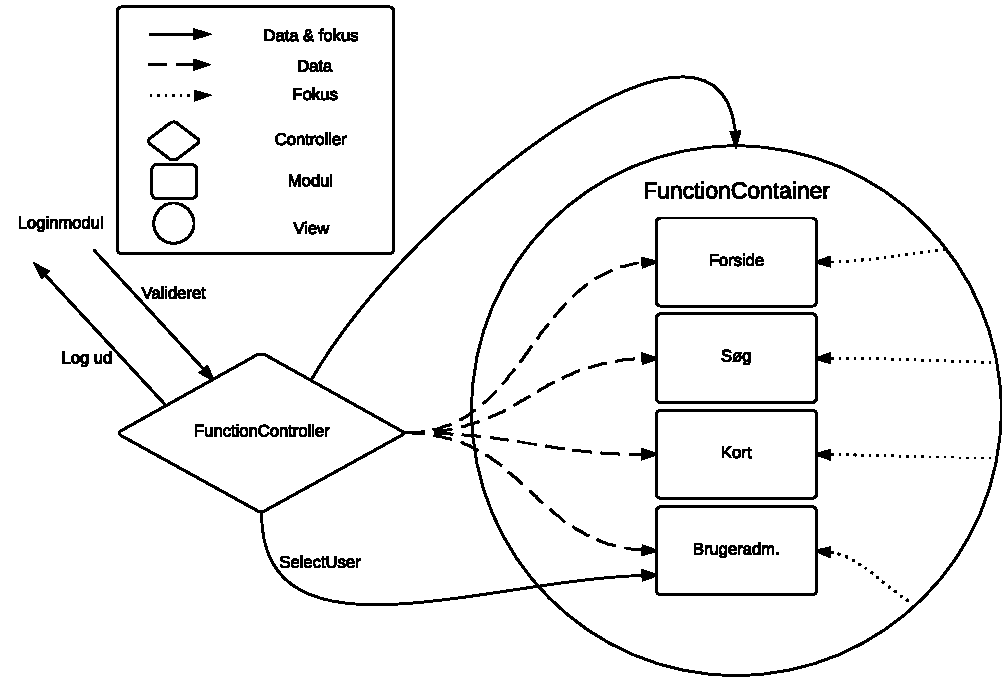
\includegraphics[width=\textwidth]{styringsmodul-diagram.pdf}
  \caption{Diagram over funktionsstyringsmodulet}
\end{figure}

Funktionsstyringsmodulet implementeres som en tabcontroller, der tilføjer andre moduler som faneblade. Default fanebladet er forsidemodulet. Dertil tilføjer funktionsstyringsmodulet et kortmodul, et brugeradministrationsmodul samt et søgningsmodul. Disse moduler bliver dog kun tilføjet, hvis brugeren som er logget ind, har de nødvendige tilladelser. Når brugeren ønsker at forlade programmet, logges der ud, og brugeren sendes tilbage til loginmodulet. Funktionsstyringsmodulet indeholder også en metode, kaldet \enquote{SelectUser} der tager en bruger som parameter. Ved metodekald vises brugeradministrationsmodulet, med informationer omkring den bruger, der blev givet som parameter. 